\chapter{Simulation Study} \label{chap:simulation}

\section{Conditions}

A simulation study was conducted to assess three attributes of the bayesian implementation of the GLLAMM, for dichotomous outcomes:
%
\begin{enumerate}
	%
	\item \textbf{Performance.} The study assessed the performance of the MCMC chains, in terms of achieving stationarity, convergence and good mixing,  under centered (CP) and non-centered parametrization (NCP), respectively.
	%
	\item \textbf{Recovery capacity.} The study evaluated the capacity to recover the parameters of interest, e.g. regression parameters, latent variables and loadings. However, it centered its focus on the recovery of the regression parameters, as they are highly relevant for making appropriate inferences at the individual level.
	%
	\item \textbf{Retrodictive accuracy.} The study appraised the capacity of the implementation to retrodict the data of interest.
	%
\end{enumerate} 

\noindent In this context, a fully crossed design with $3 \times 2 \times 2$ experimental conditions was proposed. 

First, the author used three different samples sizes to generate the data under analysis: $500$, $250$, and $100$. The literature on IRT models present several implementations with samples sizes above $250$, however, few present samples lower than that. The author decided to use a sample size of a $100$ to fill in this gap. Moreover, the decision was also supported by the notion that the change of the posterior sampling geometries could benefit the performance and recovery capacity of the implementation, under this setting.

Second, as expected, the author used two parametrization of the models: CP and NCP. To the author's knowledge, the IRT literature do not use the change of posterior sampling geometries, as an alternative to improve the performance of the bayesian implementation of said models. This research is set to fill in part of this gap.

Third, the author evaluated the performance, recovery capacity and retrodictive accuracy of a first-order and second-order latent variable models (FOLV and SOLV, respectively). The decision was based on the literature of Confirmatory Factor Analysis (CFA), where before fitting a SOLV model (figure \ref{fig:SOLV_model}), the researcher need to asses if the correlation structure at the first level of the FOLV model (figure \ref{fig:FOLV_model}) justifies the decision.

Therefore, ten ($10$) data sets were generated for each study condition, following the algorithm in section \ref{sub_sect:algorithm}. Each data set resembled responses to $25$ binary scored items, conforming to the SOLV model defined in figure \ref{fig:SOLV_model}. The model was motivated by the hypothesized structure for the reading comprehension sub-test, from the Peruvian public teaching career national assessment (see chapter \ref{chap:application}). The latent structure, regression parameters and loadings remained unchanged throughout the simulation replicas to reduce experimental error \cite{Kieftenbeld_et_al_2012}. 

%%%%%%%%%%%%%%%%%%%%%%%%%%%%%%%%%%%%%%%%%%%%%%%%%%%%%%%%%%%%%%%%%%%%%%%

\section{Algorithm} \label{sub_sect:algorithm}

Each data replication was simulated following a six-step procedure. First, the author randomly simulated a collection of pseudo-covariates $\mathbf{W}_{\theta}$, motivated by a similar information set present in the reading comprehension sub-test. The generated covariates were: (i) a binary ``gender" variable, describing males and females, (ii) an integer ``age" variable with range $[30, 65]$, the latter corresponding to the age of retirement, (iii) a three-level categorical ``education" variable, indicating the type of education the individual received: institute only, university only, or both; and finally (iv) a four-level categorical ``experience" variable, denoting the individual's years of work experience, where the higher the category, the higher the individual's years of experience. Associated with these, the author defined their regression parameters $\mathbf{\Gamma}_{\theta}$ where: (i) $\Gamma_{gender} = [\gamma_{m}, \gamma_{f}] = [0, 1]$, for males and females, respectively; (ii) $\Gamma_{age} = -0.01$, indicating that the individuals loose ability with age, in a linear manner; (iii) $\Gamma_{edu} = [\gamma_{io}, \gamma_{uo}, \gamma_{b}] = [-0.5, 0.5, 0]$, assuming individuals with university degree have better ability levels, followed by individuals with both educations, and last individuals with institute degrees; (iv) $\Gamma_{exp} = [\gamma_{0y}, \gamma_{5y}, \gamma_{10y}, \gamma_{11+y}] = [-0.5, 0, 0.35, 0.5]$, implying experience has decreasing returns on abilities; and finally (v) $\Gamma_{0} = 0$, indicating the absence of an intercept;  

Second, the study simulated the second- and first-order latent variables, corresponding to the reading comprehension ability and its three sub-dimensions: literal, inferential and reflective. Reading comprehension ($\theta^{(3)}_{j}$) was generated from a normal distribution $N( \mu^{(3)}_{j}, \sigma^{(3)}_{\theta} )$, with $\mu^{(3)}_{j} = \pmb{\Gamma}_{\theta} \; \mathbf{W}_{\theta}$, i.e. the linear combination of the simulated covariates and its corresponding regression parameters, and $\sigma^{(3)}_{\theta}=0.5$. On the other hand, the three sub-dimensions were generated from a multivariate normal distribution $MVN( \mu^{(2)}_{j.} , \Sigma^{(2)})$, with $\mu^{(2)}_{j.} = [\lambda^{(2)}_{1} \theta^{(3)}_{j}, \; \lambda^{(2)}_{2} \theta^{(3)}_{j}, \; \lambda^{(2)}_{3} \theta^{(3)}_{j} ]$, and $\Sigma^{(2)} = S^{(2)} R^{(2)} S^{(2)}$. To ensure the FOLV model in figure \ref{fig:FOLV_model} lead us to the SOLV in figure \ref{fig:SOLV_model}, the author assumed loadings $[\lambda^{(2)}_{1}, \lambda^{(2)}_{2}, \lambda^{(2)}_{3}] = [0.95, 0.95, 0.95]$. Finally, $S^{(2)} = \sigma^{(2)}_{\theta} I$, i.e a diagonal standard deviation matrix with $\sigma^{(2)}_{\theta} = 0.5$; whereas $R^{(2)} = I$, i.e an identity correlation matrix, implying the sub-dimensions are independent after accounting reading comprehension.

Third, the author defined five ($5$) common stimulus or texts for the items, where the mean difficulty for the texts $\pmb{\eta}^{(3)} = [\eta^{(3)}_{1}, \eta^{(3)}_{2}, \eta^{(3)}_{3}, \eta^{(3)}_{4}, \eta^{(3)}_{5}] = [-1.50, -0.75, 0, 0.75, 1.50]$; whereas the deviation from said mean difficulties were $\sigma^{(3)}_{\eta} = 0.5$ for all texts. 

Fourth, $25$ items were randomly generated from independent normal distributions $N( \mu^{(2)}_{k}, \sigma^{(2)}_{k} ) $, with $\mu^{(2)}_{k} = \pmb{\eta}^{(3)} \mathbf{A}$ and $\sigma^{(2)}_{k} = \sigma^{(3)}_{\eta}$, where $\mathbf{A}$ is a block design matrix that maps the items to its corresponding passage defined in the previous step. Finally, we generated at random the dimensions the items were designed to measure.

Fifth, the author calculated the linear predictor $v_{jkd}$ and probability of endorsing an item $\pi_{jkd}$, according to equations (\ref{eq:linear_predictor2}), (\ref{eq:systematic}), and (\ref{eq:response_dich1}), respectively. The probabilty was calculated using the logit inverse-link function.
	
Sixth and last, the outcome $y_{jkd}$ was simulated from a Bernoulli distribution as in equation (\ref{eq:distributional}), with its probability calculated in the previous step.

The code associated with the full simulation process can be found in Appendix \ref{appC2_1:sim}.

%%%%%%%%%%%%%%%%%%%%%%%%%%%%%%%%%%%%%%%%%%%%%%%%%%%%%%%%%%%%%%%%%%%%%%%
%%%%%%%%%%%%%%%%%%%%%%%%%%%%%%%%%%%%%%%%%%%%%%%%%%%%%%%%%%%%%%%%%%%%%%%

\section{Evaluation criteria}

La precisión de los estimados fue evaluada usando la Raíz del Error Cuadrático Medio (RMSE) y el Error Absoluto Medio (MAE) para cada réplica (acorde con los diseños establecidos en \ref{sec:cond_simulacion}). \\

El RMSE es definido como la raíz cuadrada del promedio de las diferencias entre los valores reales y los estimados al cuadrado, de la siguiente manera:
\begin{align}
	%
	RMSE \left( \eta^{(m)}_{kd} \right) &=\sqrt{\frac{1}{R} \sum_{r=1}^{R} (\hat{\eta}^{(m)}_{kd} - \eta^{(m)}_{kd} )^2} \\
	%
	RMSE \left( \theta^{(l)}_{jd} \right) &=\sqrt{\frac{1}{R} \sum_{r=1}^{R} (\hat{\theta}^{(l)}_{jdr}-\theta^{(l)}_{jd})^2}
	%
\end{align}

Tal y como se observa en las fórmulas, los criterios serán aplicados a los parámetros de ítem e individuos. Sin embargo, dado que en el NRM, el impacto de cada categoría depende ampliamente de los valores y comportamiento de las otras, en determinados casos se podría observar diferencias entre el parámetro real y estimado que no necesariamente corresponderían con un error en la estimación de la elección de la categoría por parte del individuo \citep{Wollack2002}. Así, para corregir este inconveniente se comparará no solo los estimados de los parámetros de los ítems e individuos, sino también las probabilidades condicionales asociadas a la elección de cada alternativa específica \cite{Yen_1987, Wollack_2002}. De este modo, dado que las probabilidades $P_{jk}(\theta_{i})$ difieren entre sí, no solo por los parámetros de los ítems ($a_{jk}$ y $c_{jk}$) sino también en función de las habilidades ($\theta_i$), para el análisis de las diferencias entre las probabilidades estimadas y las reales, se planteó utilizar los dos criterios (RMSE y MAE) con algunos ajustes:

\begin{align}
	%
	RMSE \left( \pi_{jkd} \right) &=\sqrt{ \frac{1}{n} \sum_{i=1}^{n} \left[ \frac{1}{R} \sum_{r=1}^{R} (\hat{\pi}_{jkdr} - \pi_{jkd})^2 \right]} \\
	%
\end{align}

\noindent donde $\hat{\pi}_{jkdr}$ es el estimado de las probabilidades condicionales en la réplica $r = 1, \dots, R$.\\

\noindent Como se observa en las formulas $(4.7)$ y $(4.8)$, las diferencias entre probabilidades se agregan y promedian a nivel de replicas y posteriormente a nivel de individuos en cada una de las réplicas ($R=20$). De esta manera, se tienen una medida global de ajuste a los datos. \\


additionally we are going to use predictive accuracy, sensitivity and the other
binary case. Based on a confussion matrix 


%%%%%%%%%%%%%%%%%%%%%%%%%%%%%%%%%%%%%%%%%%%%%%%%%%%%%%%%%%%%%%%%%%%%%%%
%%%%%%%%%%%%%%%%%%%%%%%%%%%%%%%%%%%%%%%%%%%%%%%%%%%%%%%%%%%%%%%%%%%%%%%

\section{Results}

following the CFA model construction we are going to evaluate two models that can be considered equivalent 
%
\begin{figure}[h]
	\centering
	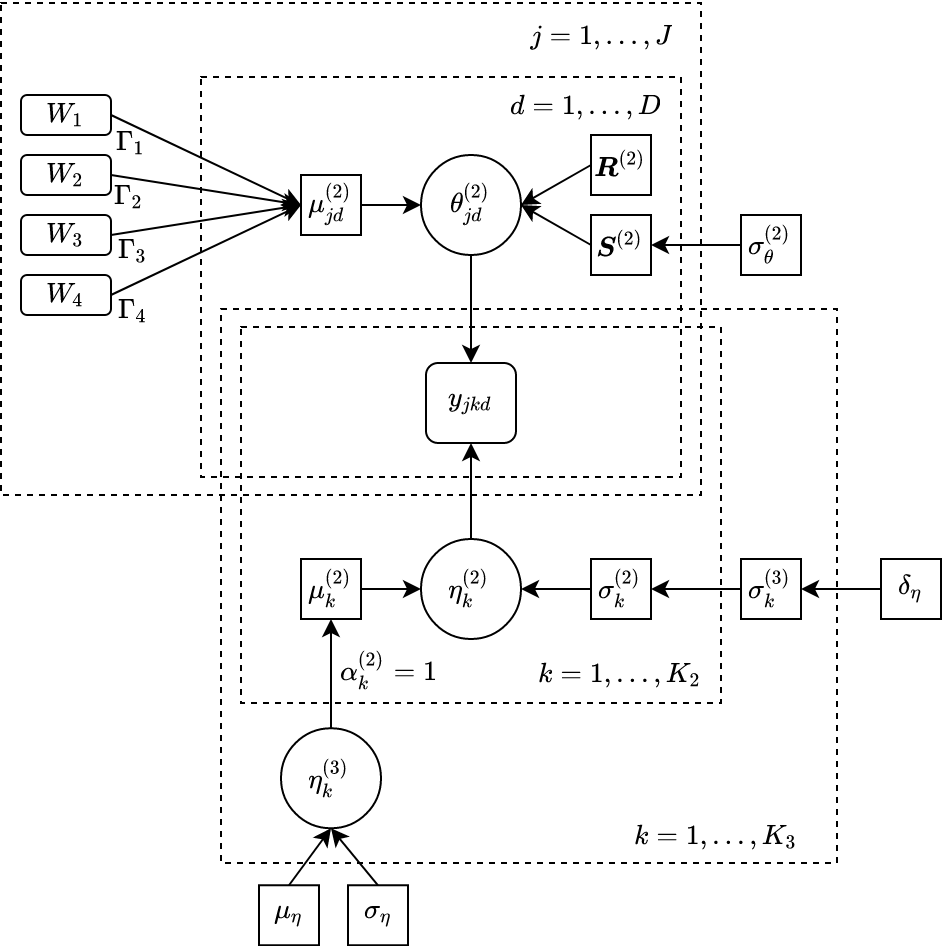
\includegraphics[width=0.7\linewidth]{4_FOLV_dag}
	%
	\caption[Directed Acyclig Graph (DAG). First Order Latent Variables model (FOLV).]%
	{Directed Acyclig Graph (DAG). First Order Latent Variables model (FOLV). Circles represent latent variables. Squares represent parameters for priors. Large Squares represent nesting in specific units.}
	\label{fig:FOLV_model}
\end{figure}
%
\begin{figure}[h]
	\centering
	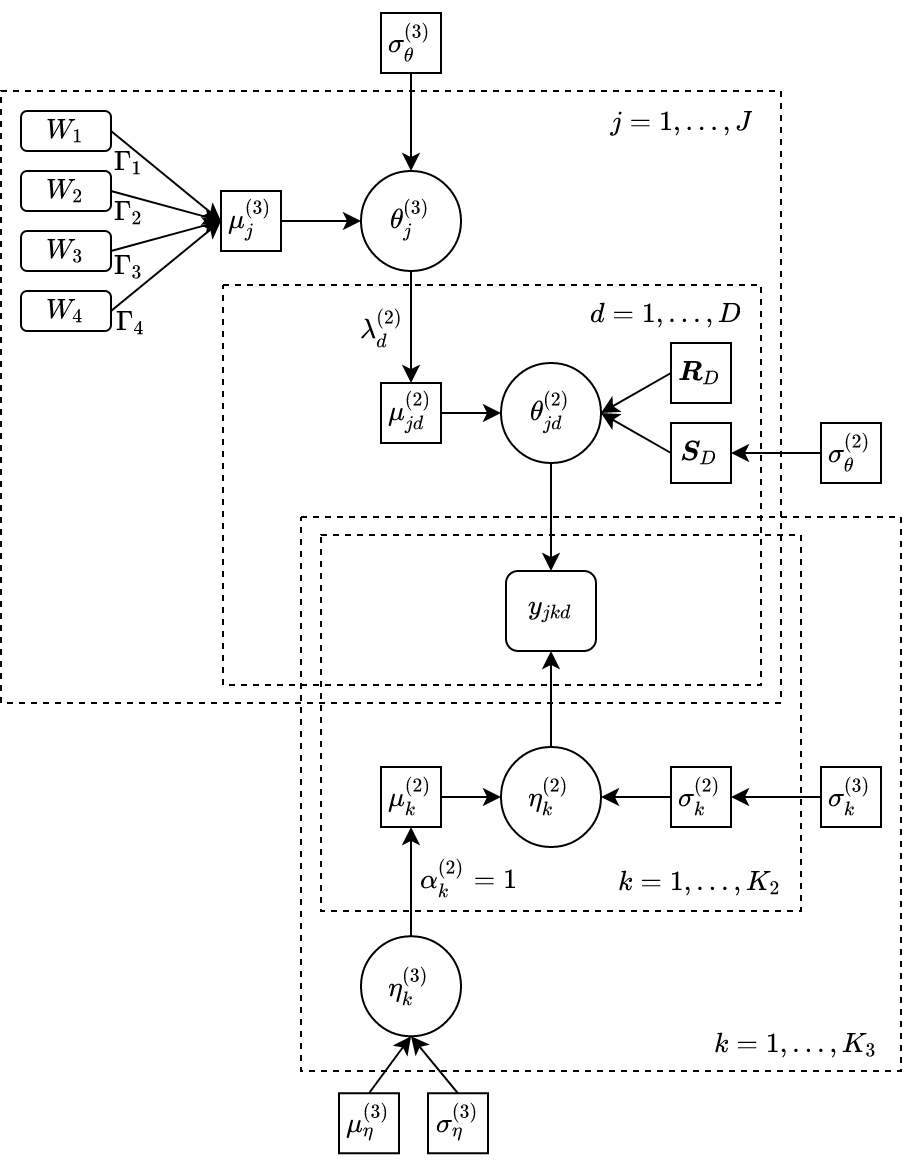
\includegraphics[width=0.7\linewidth]{4_SOLV_dag}
	%
	\caption[Directed Acyclic Graph (DAG). Second Order Latent Variables model (SOLV).]%
	{Directed Acyclig Graph (DAG). Second Order Latent Variables model (SOLV). Circles represent latent variables. Squares represent parameters for priors. Large Squares represent nesting in specific units.}
	\label{fig:SOLV_model}
\end{figure}

\subsection{FOLV CP}

\subsection{FOLV NCP}

\subsection{SOLV CP}

\subsection{SOLV NCP}

